
\section{Experiment}

\label{sec:experiment}

\subsection{Implementation Details}
\textbf{Dataset and  Metric}
We conduct experiments using benchmark datasets of TensorIR Synthetic \cite{jin2023tensoir}, DTU \cite{jensen2014large} and Mipnerf-360 \cite{barron2022mipnerf360} to evaluate our method's performance on both synthetic and real-world scene. We evaluate the
synthesized novel view and relighting results in terms of Peak
Singal-to-Noise Ratio (PSNR), Structural Similarity Index Measure (SSIM), and Learned Perceptual Image Patch Similarity (LPIPS).
\textbf{Baselines}
Considering the popularity and
performance, we selected NeRFactor \cite{zhang2021nerfactor}, NeRFdiffRec \cite{munkberg2022NVDiffrec}, Invrender \cite{invrender}, TesnorIR\cite{jin2023tensoir}, Relightable 3DGS\cite{gao2023relightable} and GSIR \cite{liang2023gsir} as our main competitor.
We conducted a comprehensive comparison between the aforementioned methods and our approach in terms of efficiency and quality. Our method are conducted on a single NVIDIA GeForce RTX 3090 GPU. 
\subsection{Results on Synthetic Datasets}
We compare our method with previous state-of-the-art offline and real-time relighting methods. Table \ref{tab_main} shows that our method outperforms both previous offline and real-time methods on Novel view synthesis. Our relighting results rank first in all real-time methods and second in all methods, only behind TensoIR. Taking both efficiency and quality into account, our approach achieves optimality. Figure \ref{main} shows visual results on Relighting tasks. We test our method under different lighting conditions and our method performs well on all lighting conditions with visually appearing results. Furthermore, we also test our method on composite synthetic scenes like \cite{gao2023relightable} and the result shows that our method can not only facilitate material editing like \cite{jin2023tensoir,liang2023gsir,shi2023gir} but also support scene editing and generate photo-realistic results and soft shadow. 
\begin{figure}[htbp]
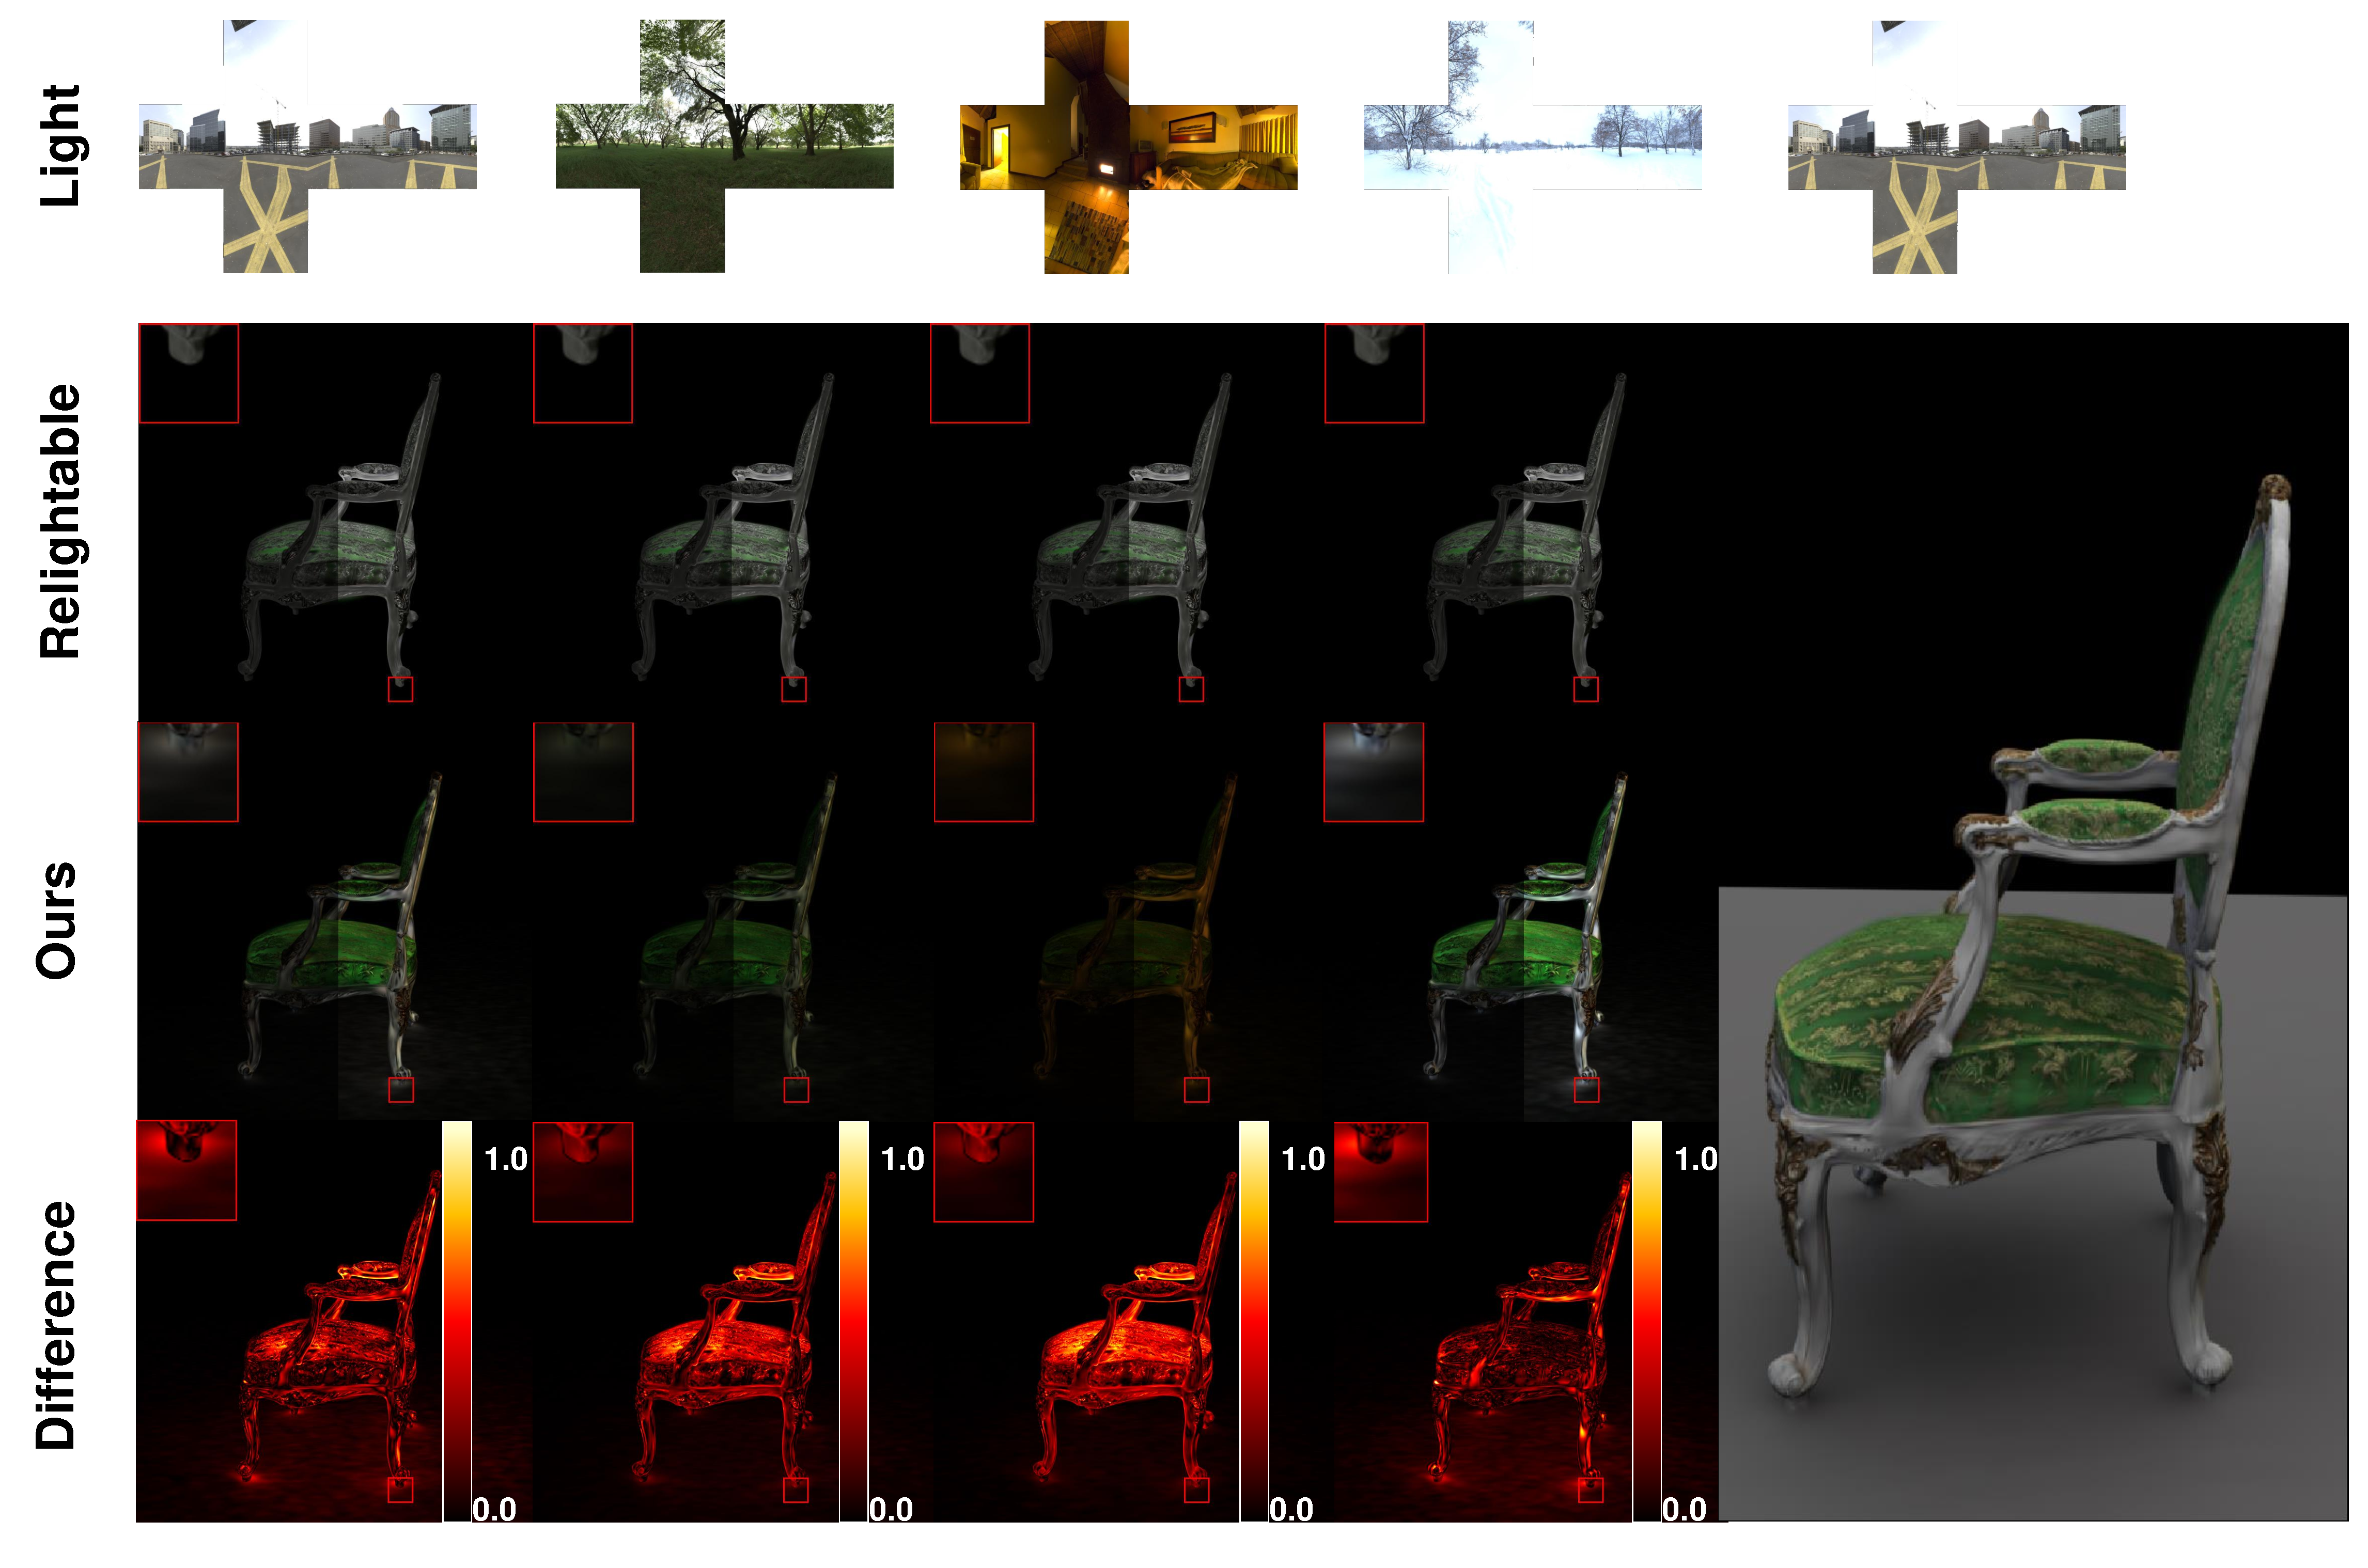
\includegraphics[width=\linewidth]{figures/indir4.pdf}
\centering
\vspace{-0.4cm}
\caption{Qualitative comparison on TensoIR Synthetic dataset. We visualize the indirect illumination in different lighting conditions. To showcase more details, we have merged the doubled-scaled indirect illumination results (on the right half) with the original brightness indirect illumination results (on the left half). The top-left corner exhibits a magnified view of the local area.}\label{indir}
\vspace{-0.4cm}
\end{figure}

\begin{table}[htbp]
 \vspace{-0.3cm}
  \centering
      \caption{Quantatitive Comparison on Mip-NeRF 360. Our method surpasses most NeRF variants and Gaussian inverse rendering method dedicated to novel view synthesis}
    \begin{tabular}{c|ccc}
    \hline
     Method&PSNR$\uparrow$&SSIM$\uparrow$&LPIPS$\downarrow$\\
    \hline
     NeRF++& 26.214& 0.659 &0.348\\
    Plenoxels&  23.625& 0.670& 0.443\\
    INGP-Base&  26.430& 0.725 &0.339\\
    Gsir& 26.659 &0.815 &0.229\\
    Ours& \textbf{28.116}&\textbf{0.865}&\textbf{0.182}\\
    \hline
    \end{tabular}%
 \vspace{-0.7cm}
  \label{mip}%
\end{table}%


%我们比较了低光脉冲流和增强脉冲流的重构结果。为了充分说明我们的增强脉冲流能有效地改善低光脉冲流的质量，我们测试了最先进的重构算法xxx，xxx和xxx。此外，两种低光高速脉冲流数据集xxxandxxx被评估.其中xxx主要针对室内场景而xxx关注室外场景。%由于真实数据集缺少高帧率(20,000 Hz)场景图像作为gt, 我们使用了三种无参考指标去评估方法性能, i.e., MA[],  BRISQUE[] and NIQE[].
\subsection{Results on real-world Datasets}
We extend our evaluation to real-world dataset \cite{barron2022mipnerf360,jensen2014large} with geometric intricacies inherent and complex lighting conditions. Due to the lack of data under varying lighting conditions, Tab \ref{mip} only presents the quantitative comparisons on real-world datasets on Novel view synthesis tasks. From Tab \ref{mip} we can conclude that our real-time relighting approach even surpasses most NeRF variants and the advanced inverse rendering method dedicated to novel view synthesis. Figure \ref{main} demonstrates reconstructed scene details including high-frequency appearance, rendering high-fidelity appearance, and recovering fine geometric details.


%如表所示,我们的方法取得了很好地性能。具体地，我们分别使用增强脉冲流和低光脉冲流接入LS2ES，来自增强脉冲流的重构图像的质量将大大提高。图x展示了可视化结果。我们可以看到增强脉冲流不仅仅改善了场景亮度信息并且使得重构结果更加清晰。


%We can find that the enhanced spike streams not only improve the scene brightness information but also make the results clearer.

% Table generated by Excel2LaTeX from sheet 'Sheet1'




% \begin{table*}[htbp]
%   \centering
%   \caption{Ma, Brisque and Niqe of reconstruction on the dataset, LLSD. $d_{1-4}$ denotes $drive_1$, $drive_2$, $drive_3$ and $drive_4$ on LLSD. }
%     \resizebox{2\columnwidth}{!}{
%     %  \begin{tabular}{c|ccc|ccc|ccc|ccc|ccc|ccc|ccc|ccc}
%     \begin{tabular}{c|cc|cc|cc|cc|cc|cc|cc|cc}
%      % \Xhline{1.5px}
%     \hline
%     Method&\multicolumn{8}{c|}{Novel View Synthesis} & \multicolumn{8}{c}{Relight}\\
%     \hline
%     Scene&
%     \multicolumn{2}{c|}{armadillo}& \multicolumn{2}{c|}{ficus}& \multicolumn{2}{c|}{lego} & \multicolumn{2}{c|}{avg} &
%     \multicolumn{2}{c|}{armadillo}& \multicolumn{2}{c|}{ficus}& \multicolumn{2}{c|}{lego} & \multicolumn{2}{c}{avg}\\
%     Metircs&PSNR&SSIM&PSNR&SSIM&PSNR&SSIM&PSNR&SSIM&PSNR&SSIM&PSNR&SSIM&PSNR&SSIM&PSNR&SSIM\\
%     \hline
%     NeRFactor  & 26.479 &0.947& 21.664& 0.919&  
%         26.076& 0.881& 24.740& 0.916&
%          26.887 & \cellcolor {yellow!20}0.944 &20.684& \cellcolor {pink!70}0.907&
%          23.246 &\cellcolor {yellow!20}0.865& 23.606& \cellcolor {pink!70}0.908\\
%     InvRender  & 31.116 & 0.968 & 22.131 &0.934&
%         24.391 &0.883&  25.879& 0.928&
%          \cellcolor {yellow!20}27.814 &\cellcolor {pink!70}0.949 & 20.330& \cellcolor {yellow!20}0.895&
%           20.117& 0.832& 22.754 &0.892\\
%     NVDiffrec  &33.664  &\cellcolor {yellow!20}0.983 & 22.131& 0.946& 
%         30.056& 0.945&  28.617 &0.958&
%          23.099 &0.921& 17.260& 0.865&
%          20.088& 0.844 & 20.149 &0.877\\
%     TensoIR  &\cellcolor {yellow!20}39.050 & \cellcolor {pink!70}0.986 & \cellcolor {yellow!20}29.780 &\cellcolor {yellow!20}0.973& 
%         \cellcolor {pink!70}34.700& \cellcolor {pink!70}0.968&  \cellcolor {yellow!20}34.540&\cellcolor {yellow!20} 0.976&
%          \cellcolor {red!40} \textbf{34.504}& \cellcolor {red!40} \textbf{0.975}& \cellcolor {yellow!20}24.296 &\cellcolor {red!40} \textbf{0.947}&
%          \cellcolor {red!40} \textbf{28.581}& \cellcolor {red!40} \textbf{0.944}& \cellcolor {red!40} \textbf{29.127}& \cellcolor {red!40} \textbf{0.955}\\
%     Gsir   &\cellcolor {pink!70}39.287 & 0.980 &  \cellcolor {pink!70}33.551 &\cellcolor {pink!70}0.976& 
%         \cellcolor {yellow!20}34.379 &\cellcolor {pink!70}0.968& \cellcolor {pink!70}35.739 &\cellcolor {pink!70}0.975&
%          27.737 &0.918& \cellcolor {pink!70} 24.932 &0.893&
%         \cellcolor {yellow!20} 23.256& 0.842 & \cellcolor {yellow!20}25.308 &0.884\\
%     Relightable\_3dgs  &33.664  &\cellcolor {yellow!20}0.983 & 22.131& 0.946& 
%         30.056& 0.945&  28.617 &0.958&
%          23.099 &0.921& 17.260& 0.865&
%          20.088& 0.844 & 20.149 &0.877\\
%     Ours & \cellcolor {red!40} \textbf{46.917}& \cellcolor {red!40} \textbf{0.991}& \cellcolor {red!40} \textbf{41.207}&\cellcolor {red!40} \textbf{0.994} &
%     \cellcolor {red!40} \textbf{37.830}&\cellcolor {red!40} \textbf{0.980} & \cellcolor {red!40} \textbf{41.985}&\cellcolor {red!40} \textbf{0.988} & 
%     \cellcolor {pink!70}32.53 &  0.943& \cellcolor {red!40}26.73 & 0.888 
%     &\cellcolor {pink!70} 24.02 & \cellcolor {pink!70}0.879& \cellcolor {pink!70}27.76&\cellcolor {yellow!20}0.903 \\ 
%      % \cline{12-15}\cline{4-7}\cline{8-11}
%     \hline
%     \end{tabular}%
%    }
%   \label{tensoir}%
% \end{table*}%






%Additionally, in Fig.~\ref{rec_LLSD}(c), the shock absorber of the electromobile is clearly reconstructed, while the reconstruction results from the low-light spike stream lose the relevant information.
%我们评估了增强框架LS2ES在LLSD四类驾驶场景()中的表现。如表所示, 我们的方法能有效地增强低光脉冲流。来自增强脉冲流的重构图像的质量得到了大幅度的改善。Figure.~\ref{} shows four the visual results 分别来自x，x，x和x. We can find that the enhanced spike streams not only improve the scene brightness information but also make the reconstruction results clearer. 具体地，车牌上的字能被更容易地认出 in Fig(a). 此外，in Fig(c)，电动车的减震器被清晰地重构出来了而低光脉冲流的重构结果中缺少相关细节信息.
\subsection{Ablation}
%To investigate the effect of the proposed light-robust representation LR-Rep, the \textbf{a}djacent (forward and backward) \textbf{d}eep temporal \textbf{f}eatures (ADF), \ie  $\mathbf{F}_{t_i}^b$ and $\mathbf{F}_{t_i}^f$ in our fusion module, the \textbf{a}lignment \textbf{i}nformation in our \textbf{f}usion module (AIF) and GISI transform in LR-Rep, we compare 5 baseline methods with our final method. (A) is the basic baseline without LR-Rep, ADF and AIF. Table.~\ref{ablation} shows ablation results on proposed dataset, LLR. The comparison between (A) and (C) ((B) and (D)) proves the effectiveness of LR-Rep. The comparison between (A) and (B) ((C) and (D)) proves the effectiveness of ADF. Further, by adding the alignment information in the fusion module \ie AIF, our final method (F) appropriately reduces the misalignment of motion from different timestamps and can reconstruct high-speed scenes more accurately than (D). Besides, the comparison between (E) and (F) shows GISI has better performance than LISI. It is because GISI can extract more temporal information than LISI (see Fig.~\ref{gisi_lisi}).






%我们的增强框架包括两个部分一个是网络另一个是解码器，下面我们将分别讨论他们对性能的影响。

\textbf{Indirect illumination}
To demonstrate the effectiveness of our indirect illumination model, we conducted comparisons with two alternative variants: a model without indirect illumination (w/o indirect) and a model with ambient occlusion indirect illumination (AO indirect). We report the average scores on the TensoIR dataset, as outlined in Tab \ref{indirect_tap}. Our analysis reveals that accurate indirect illumination plays a pivotal role in estimating accurate material decomposition and producing photorealistic rendering results. To prove that our raytracing and indirect illumination estimation method can compute accurate indirect illumination related to environment light, we compare our method with Relightable 3DGS \cite{gao2023relightable} in different lighting conditions. Figure \ref{indir} shows that the indirect illumination generated by our method not only adapts to lighting conditions but also adjusts with changes in the scene.
\begin{table}[htbp]
 \vspace{-0.3cm}
  \centering
        \caption{Analyses on the impact of indirect illumination. }
         \vspace{-0.3cm}
    \resizebox{1.0\linewidth}{!}{
    \begin{tabular}{c|ccc|ccc}
    \hline
    \multirow{2}{*}{Method}& \multicolumn{3}{c|}{TensoIR Synthetic}& \multicolumn{3}{c}{DTU}\\
    \cline{2-7}
    &PSNR$\uparrow$&SSIM$\uparrow$&LPIPS$\downarrow$&PSNR$\uparrow$&SSIM$\uparrow$&LPIPS$\downarrow$\\
    \hline
     AO indirect& 38.681 & 0.981 & 0.024
                &29.192&0.933&0.108\\
    w/o indirect&  39.122 &0.983& \textbf{0.022} 
                &29.301&0.934&0.108\\
    Ours& \textbf{41.985}& \textbf{0.988}& \textbf{0.022}
                &\textbf{29.458}&\textbf{0.935}&\textbf{0.107}\\
    \hline
    \end{tabular}%
}
 \vspace{-0.5cm}
  \label{indirect_tap}%
\end{table}%





\hupar{Spherical Harmonics Order} We investigate the impact of Spherical Harmonics Order on the relighting quality. We select orders 2, 3, and 6 and report the quantitative results on Tap \ref{tab_sh}. Our analysis indicates that under relatively smooth environmental lighting conditions, the order of spherical harmonic functions has a minor impact on the quality of results but a significant effect on rendering speed. 
%对于脉冲流的超分，我们使用最先及的深度学习方法[]在LLSD上进行评估.注意，由于LLSD本身脉冲流的空间分辨率是高的(1000x1000), 我们从中心将其空间分辨率剪裁为256x256。fig展示了可视化结果。我们能发现增强脉冲流能使超分结果中恢复更多纹理细节。

\begin{table}[htbp]
  \centering
  \vspace{-0.1cm}
        \caption{Analyses on the impact of SH order. SH order has little influence on relighting quality.}
     \vspace{-0.3cm}
        \begin{tabular}{c|ccc|c}
    \hline
    Method&PSNR $\uparrow$& SSIM $\uparrow$& LPIPS $\downarrow$ &Render time\\
    \hline
     SH Order 2& {27.730} & 0.904 &0.073& {0.012}\\
    SH Order 3&  27.722 & 0.904& 0.073&0.013\\
    SH Order 6&  27.720 & 0.904 &0.073&0.050\\
    \hline
    \end{tabular}%
 \vspace{-0.6cm}
  \label{tab_sh}%
\end{table}%



%For the second scene, the OF from the low-light spike stream (upper right corner) has the wrong direction of motion. 
%We can find that enhanced spike streams effectively improve the above problems and help to predict optical flow more accurately.
%对于LLSD, 全部场景都在运动时被拍摄. 然而，对于第一个场景，光流from低光脉冲没有预测出背景的运动. 对于第二个场景, 光流from低光脉冲(右上角)有着错误的运动方向。我们能发现增强脉冲流使得有效地改善上述情况and帮助更准确地预测光流。
% Table generated by Excel2LaTeX from sheet 'Sheet1'